\documentclass{article}
\usepackage{listings}
\usepackage{graphicx}
\usepackage{float}
 
\floatstyle{ruled}
\newfloat{program}{thp}{lop}
\floatname{program}{Snippet}


\begin{document}

\title{Project Report - Limited Static Type Checking for JavaScript}
\author{Huascar A. Sanchez \and Tim Disney}

\maketitle

\lstset{showstringspaces=false}

\section{Introduction}
It is well known that in the construction of software it is generally cheaper to 
catch programming errors earlier in the development cycle \cite{cc2}. One method 
of catching these errors is static type checking. As we all know with static type 
checking, the type consistency of your code will be checked before the program is 
run. In other words, if there are any type violation in your code the the type 
checker will catch it. 

For example, invoking a method on an object that does not support it will be easily 
detected in strongly typed languages like Java. The compiler will immediately 
complain and will prevent the program from running. However, in languages like 
JavaScript, this type of error will be overlooked and deffered until runtime.

Enabling static type checking in a language as dynamic as JavaScript is a 
challenge. Especially since types can be modified at runtime. Given this constraint, 
we implemented a static type checker, called JSCheck, for prototype based objects 
in JavaScript. The scope of our checker was limited to properties on objects' 
prototype. In other words, we are completely ignoring type checking of things 
like strings and numbers. The whole idea, as Lucas Cardelli said \cite{typesystems}, 
is to prevent the occurance of execution errors during the running of your program. 

Our implementation is both unsound and incomplete. One thing that sets our 
implementation apart for previous work is that our checker works (in a limited 
fashion) for full JavaScript.

The rest of this paper is divided as follows. The implementation section will discuss 
any design and implementation choices that were made throughout the development 
of this static type checker. A collection of snippets is provided to show our checker 
in action. Our findings and conclusions will be discussed in the last section of 
this paper.

\section{Implementation}
JSCheck is a static type checker for prototype based objects in JavaScript. It uses 
explicit type annotations, written in your comments, to determine what to type check 
in a given user-defined function (see Snippet 1). It was implemented in Haskell 
\cite{haskellLanguage}. It uses a modified version of the JavaScript grammar that 
supports type annotations. It uses the HJS library \cite{hjsLibrary} to parse 
JavaScript code, which complies with ECMAScript 3rd edition plus some additions 
from JavaScript 1.5. 

\begin{program}
\begin{verbatim}
function Dog() {
  //..
}

Dog.prototype.getName = function(){
  //..
}

Dog.prototype.bark = function(){
  //..
}

//# @type Dog fido
function useDog(fido) {
  fido.bark();
}

var d = new Dog();
useDog(d);
\end{verbatim}
\caption{Type Checking}
\end{program}

Unless you explicity type annotate your functions, JScheck does not have the means 
for type checking them. The way our checker works is very straightforward. It a
three-steps process (see Figure ~\ref{fig:jscheckway}). First, it takes some JavaScript 
code and parses it. The output is an Abstract Syntax Tree (AST). Second, given this AST, 
it extracts all the possible types found in your code. The output is what we know 
as the environment. The environment is the place where type names are mapped to 
their available type fields. Third, the environment and the AST are then fed to 
a built-in type checking process. Here is where any type consistency will be checked 
and, if there are any, type consistency violations will be communicated to the 
developer. 

\begin{figure}[here]
  \begin{center}
    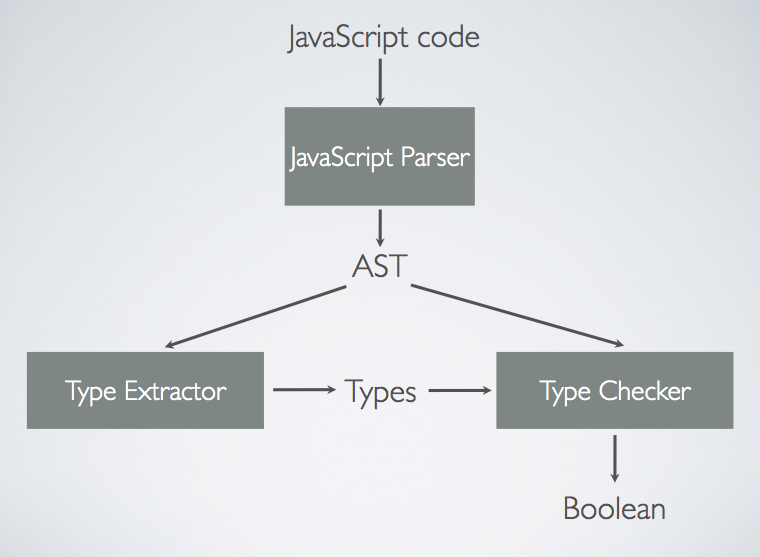
\includegraphics[scale=0.5]{blockdiagram.png}
  \end{center}
  \caption{Type Checking - the JSCheck way}
  \label{fig:jscheckway}
\end{figure}
\pagebreak



As could see in the above figure, after the code has been parsed, the JScheck will 
extract the types and check them on functions that have type annotations. The final 
output will be either your code is well-typed or not (represented as a boolean value). 
We plan on changing this output to a more descriptive one (i.e., including where the
type violation occurred, the name of the function, and a suggestion for how to fix it). 


\section{Related Work}
We are not the first ones who have tried to implement static type checking for JavaScript.
There have been others who have done it before us. Some of them include:

\begin{description}
  \item[Tom Austin and Caitlin Sadowski] \hfill \\ 
  developed a structural type-checker for Javascript \cite{fwjsStruct}.
  \item[$JS_0$ team] \hfill \\ 
  developed a formalism for an object based language called JSO, which includes features of JavaScript 
  \cite{typeinferenceforjavascriptEcoop,typecheckingforjavascript}. 
  \item[DRuby team] \hfill \\ 
  developed Diamondback Ruby (DRuby), a tool that blends Ruby's dynamic type 
  system with a static typing discipline \cite{typecheckingruby}.
  \item[Google] developed the Closure compiler \cite{closureCompiler}.  
\end{description}

In some way, which remains obscure, we all shared the same drive for making type 
checking possible in a dynamic language. We chose JavaScript for many reasons. 
However, the most important one, for us, was that JavaScript is the most used 
language in the World Wide Web and providing this type checking capability would
be appreciated by many. 

\section{Future Work}
There are several areas in our static type checker that could be expanded. One of
them, as indicated above, is the type checking output. Future will be focused on 
providing a more descriptive type checking output. Another extension could be to
provide type consistency checks for other elements of the language, like strings
and numbers.


\section{Conclusion}
We have developed a static type checker for prototype based objects in JavaScript
called JSCheck. By using this checker any developer will be able to catch any 
type errors before running their programs. The only thing the developer needs to
do is to explicitly type annotate a function(s). The rest is done by JSCheck. 

The idea of implementing a type checker strongly motivated us. It is hard for us 
describe the feeling of accomplishment after completing our implementation. Now,
for sure, we have a better understanding of what static type checking is all about. 

\bibliographystyle{abbrv}
\bibliography{report}

\end{document}


